\documentclass{beamer}
\usepackage[activeacute,spanish]{babel}
\usepackage{latexsym,cancel}
\usepackage[T1]{fontenc}
\usepackage[latin1]{inputenc}
\usepackage{amsmath}
\usepackage{amsthm}
\usepackage{amsfonts}
\usepackage{amssymb}
\usepackage[spanish]{babel}
\usepackage[latin1]{inputenc}
\usepackage{graphicx}
\usepackage{amsmath}
\usepackage{dsfont} % colocar los numeros r
\usepackage{float}
\usepackage{fancyhdr}
\usepackage{anysize}
\usepackage{booktabs}
\usepackage{multirow}
\usepackage{titlesec}
\usepackage{enumerate}
\usepackage{verbatim}
\usepackage[spanish]{babel}
\usepackage{beamerthemesplit}
\usepackage{ragged2e}
\justifying
\setbeamertemplate{background canvas}[vertical
shading][bottom=white,top=structure.fg!25]
\usecolortheme[RGB={134,0,0}]{structure}
\usetheme{Madrid}
\justifying
\decimalpoint
\title[Transformadores]{Confiabilidad y algunas pol\'iticas de inventario para transformadores de instrumento} 
%sirve para [] poner t�tulos compactos en el tema
\author[Alma Maldonado]{Alma Delia Maldonado
Santiago}

\institute[CIMAT]{
Directores: Dr. Enrique Villa Diharce.\\
Dr. Andr\'es Christen Garc\'ia.}

\date[Agosto 2013]{Agosto 2013}
\begin{document}



\maketitle
%\frame{\frametitle{Contenido} \tableofcontents}
%\section{Definici\'on del problema}
\begin{frame}
\frametitle{Definici\'on del problema}
\begin{center}
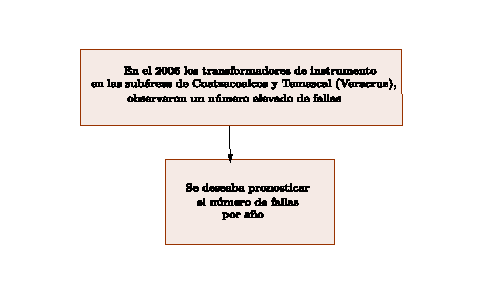
\includegraphics[scale=1.3]{def.pdf}
\end{center}
\end{frame}


\frame{\frametitle{Transformadores de instrumento}
\begin{itemize}
\justifying
\item Los transformadores de instrumento ayudan a determinar los consumos de energ\'ia. %formando parte del sistema de medici\'on de energ\'ia el\'ectrica para las redes de alta tensi\'on y con ellos realizar los montos de los  cobros. 
\item Sirven de protecci\'on, al momento en que se origina una descarga. %El sistema designado para protecci\'on desactiva los interruptores, con lo que evita que se generen da\~nos de mayor magnitud en la red.
\item Cuando el transformador falla de manera catastr\'ofica impide la medici\'on del flujo de energia el\'ectrica.
\end{itemize}
  
\includegraphics[scale=0.5]{trans.jpg}  
}

\frame{\frametitle{Objetivos}
\begin{enumerate}
\justifying
\item Revisar la teor\'ia Bayesiana necesaria para abordar el problema.
\item Proponer alguna estrategia \'optima de inventario o almacenamiento, mediante una funci\'on de utilidad que permita minimizar los costos esperados. 
\end{enumerate}
}
%\section{Metodolog\'ia}
\frame{\frametitle{M\'etodo Bayesiano para realizar inferencia}
\begin{figure}
\begin{center}
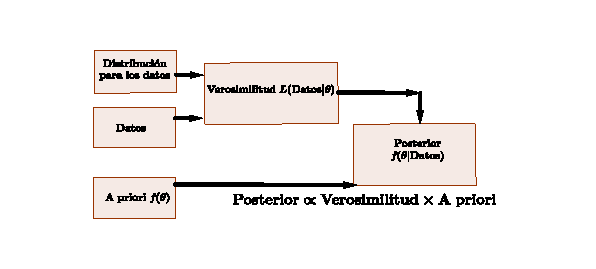
\includegraphics[scale=0.1]{bayes.pdf}
\end{center}
\end{figure}
}

\frame{\frametitle{M\'etodo Bayesiano para realizar  inferencia}
\begin{itemize}
\justifying
\item Conocimiento a priori acerca de $\theta$ expresado en t\'erminos de una funci\'on de densidad de probabilidad denotada por $f(\theta)$.
\item La verosimilitud para los datos disponibles y un modelo especificado dado por $L(Datos|\theta)$.
\item Utilizar la regla de Bayes:% para obtener una distribuci\'on posterior, que resulte de la combinaci\'on de la verosimilitud y el conocimiento de la distribuci\'on a priori de $\theta$. 
\begin{center}
\begin{tabular}{|c|}
\hline
Posterior $\propto$ A priori $\times$ Verosimilitud.\\
\hline
\end{tabular}
\end{center}

\end{itemize}
}

\frame{\frametitle{Datos}

\begin{table}[h!]\tiny
\begin{center}
%\caption {\bf Tiempos de vida de transformadores de corriente, $t_i$ (meses), $e_i=1$ indica un dato censurado, $e_i=0$ es un dato no censurado.\label{uno}}
\begin{tabular}{ccc|ccc|ccc|ccc}
\toprule[0.6mm]
$i$	&	$t_i$	&	$e_i$	&	$i$	&	$t_i$	&$e_i$	&	$i$	&	$t_i$	&	$e_i$	&	$i$	&	$t_i$	&	$e_i$	\\
\toprule[0.6mm]
1	&	8	&	1	&	36	&	107	&	0	&	106	&	272	&	1	&	141	&	308	&	0	\\
2	&	8	&	1	&	37	&	116	&	1	&	107	&	272	&	1	&	142	&	308	&	0	\\
3	&	8	&	1	&	38	&	119	&	0	&	108	&	272	&	1	&	143	&	308	&	1	\\
4	&	8	&	1	&	39	&	119	&	0	&	109	&	272	&	1	&	144	&	308	&	1	\\
5	&	8	&	1	&	40	&	139	&	0	&	110	&	272	&	1	&	145	&	308	&	1	\\
6	&	20	&	1	&	41	&	140	&	0	&	111	&	274	&	0	&	146	&	308	&	1	\\
7	&	20	&	1	&	42	&	144	&	0	&	112	&	274	&	0	&	147	&	308	&	1	\\
8	&	20	&	1	&	43	&	146	&	0	&	113	&	274	&	0	&	148	&	308	&	1	\\
9	&	20	&	1	&	44	&	146	&	0	&	114	&	275	&	0	&	149	&	308	&	1	\\
10	&	32	&	1	&	45	&	152	&	1	&	115	&	275	&	0	&	150	&	308	&	1	\\
11	&	32	&	1	&	46	&	159	&	0	&	116	&	275	&	0	&	151	&	308	&	1	\\
12	&	32	&	1	&	47	&	159	&	0	&	117	&	276	&	0	&	152	&	308	&	1	\\
13	&	32	&	1	&	48	&	159	&	0	&	118	&	281	&	0	&	153	&	308	&	1	\\
14	&	32	&	1	&	49	&	160	&	0	&	119	&	281	&	0	&	154	&	308	&	1	\\
15	&	32	&	1	&	50	&	161	&	0	&	120	&	284	&	0	&	155	&	308	&	1	\\
16	&	32	&	1	&	51	&	164	&	1	&	121	&	284	&	0	&	156	&	308	&	1	\\
17	&	56	&	1	&	52	&	167	&	0	&	122	&	284	&	0	&	157	&	308	&	1	\\
18	&	80	&	1	&	53	&	172	&	0	&	123	&	284	&	0	&	158	&	308	&	1	\\
19	&	80	&	1	&	54	&	172	&	0	&	124	&	286	&	0	&	159	&	308	&	1	\\
20	&	80	&	1	&	55	&	176	&	1	&	125	&	286	&	0	&	160	&	308	&	1	\\
21	&	80	&	1	&	56	&	183	&	0	&	126	&	286	&	0	&	161	&	308	&	1	\\
22	&	80	&	1	&	57	&	188	&	1	&	127	&	287	&	0	&	162	&	308	&	1	\\
23	&	80	&	1	&	58	&	203	&	0	&	128	&	288	&	0	&	163	&	308	&	1	\\
24	&	80	&	1	&	59	&	205	&	0	&	129	&	288	&	0	&	164	&	308	&	1	\\
25	&	80	&	1	&	60	&	214	&	0	&	130	&	288	&	0	&	165	&	308	&	1	\\
26	&	80	&	1	&	61	&	214	&	0	&	131	&	288	&	0	&	166	&	308	&	1	\\
%27	&	80	&	1	&	62	&	215	&	0	&	132	&	296	&	1	&	167	&	308	&	1	\\
%28	&	80	&	1	&	63	&	216	&	0	&	133	&	296	&	1	&	168	&	308	&	1	\\
%29	&	80	&	1	&	64	&	216	&	0	&	134	&	296	&	1	&	169	&	308	&	1	\\
%30	&	80	&	1	&	65	&	216	&	0	&	135	&	296	&	1	&	170	&	308	&	1	\\
%31	&	80	&	1	&	66	&	218	&	0	&	136	&	298	&	0	&	171	&	308	&	1	\\
%32	&	80	&	1	&	67	&	218	&	0	&	137	&	299	&	0	&	172	&	308	&	1	\\
%%33	&	94	&	0	&	68	&	218	&	0	&	138	&	300	&	0	&	173	&	308	&	1	\\
%34	&	94	&	0	&	69	&	225	&	0	&	139	&	308	&	0	&		&	308	&	1	\\
%35	&	94	&	0	&	70	&	225	&	0	&	140	&	308	&	0	&		&	308	&	1	\\
\bottomrule[0.6mm]
\end{tabular}
\end{center}
\end{table}
}



\frame{\frametitle{Verosimilitud}
\begin{itemize}
\item Representaci\'on: $(\underline{t},\underline{e})=\{t_i,e_i\}_{i=1}^n$, donde 

\[
e_i=\left\{
\begin{array}{cl}
\displaystyle 1 & \mbox{ si } t_i \mbox{ es un dato censurado},\\                                                               0     &     \mbox{ si } t_i \mbox{ es una observaci\'on completa.}  \\
\end{array}
\right.
\]
\item Verosimilitud: $t_i\sim$ Weibull$(\beta,\eta)$, luego
\begin{eqnarray*}
f(\underline{t}|\underline{e},\beta,\eta)&=& \prod_{e_i=0}\frac{\beta}{\eta}\left(\frac{t_i}{\eta}\right)^{\beta-1}\exp \left\{-\left(\frac{t_i}{\eta}\right)^{\beta}\right\}\\
& &\prod_{e_i=1}\exp\left\{-\left(\frac{t_i}{\eta}\right)^{\beta}\right\}.
\end{eqnarray*}
\end{itemize}
}
%\section{Modelo a priori}
\frame{\frametitle{Modelos a Priori}
\begin{itemize}
\justifying
\item {\bf Instrumentos de modelaci\'on:} $\beta\sim$Ga$(a_1,b_1)$ y $\eta\sim$Ga$(a_2,b_2)$
\end{itemize}

\justifying
Es de inter\'es establecer los par\'ametros para las a prioris, estos se fijar\'an con la ayuda de dos elementos:
\begin{itemize}
\justifying
\item El comportamiento de la funci\'on de riesgo de los transformadores.
\item La distribuci\'on predictiva a priori.
\end{itemize}
}
\frame{\frametitle{Funciones de riesgo para la distribuci\'on predictiva a priori}
\begin{figure}
\begin{center}
\includegraphics[scale=0.4]{r1.png}
\end{center}
\end{figure}}

\frame{\frametitle{Determinaci\'on a priori}
\begin{figure}
\hspace{-.5cm}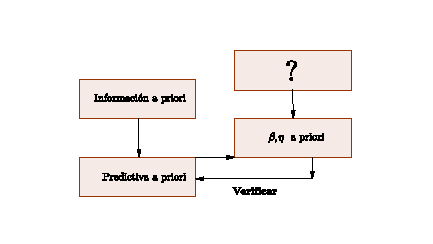
\includegraphics[scale=1.5]{aprDia.pdf}
\end{figure}
}

\frame{\frametitle{Distribuci\'on predictiva a priori}
\begin{itemize}
\justifying
\item Por experiencia  podemos conocer ciertas car\'acter\'isticas del tiempo de vida de los transformadores y tener informaci\'on de la distribuci\'on predictiva a priori. 
\item Suponiendo que el $5\%$ de los transformadores fallan en los primeros a\~nos (80 meses) y que el $95\%$ de ellos fallaron a los 40 a\~nos (480 meses) o antes. 
\end{itemize}
}



\frame{\frametitle{Distribuci\'on predictiva a priori}

\begin{figure}
\begin{center}
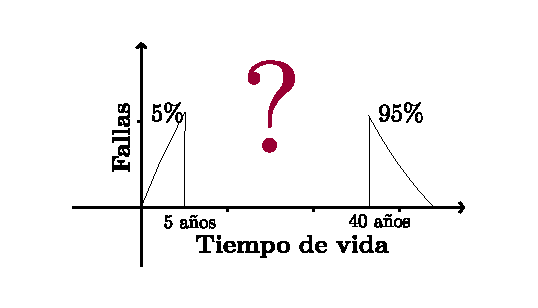
\includegraphics[scale=1.3]{apriori1.pdf}
\end{center}
\end{figure}
}

\frame{
\frametitle{Obtenci\'on distribuci\'on a priori.}
\begin{itemize}
\justifying
\item Si los tiempos de vida de los transformadores se representan por la variable aleatoria $T \sim$ Weibull $(\eta^{*},\beta^{*})$.
\item La informaci\'on anterior de los cuantiles se representa de la siguiente manera:
$$P(T\leq80)=0.05$$
$$P(T\leq480)=0.95,$$
resolviendo el sistema: $\beta^{*}=1.955$ y $\eta^{*}=273.8$
\end{itemize}
}

\frame{
\begin{itemize}
\justifying
\item De manera general la funci\'on de densidad de una variable aleatoria Gamma con par\'ametros $a$ y $s$ es:
$f(x)=\frac{1}{s^a \Gamma(a)}x^{a-1}\exp\{x/s\}$, su valor esperado es $E(X)=as.$
\item Luego $\beta^{*}=1.955\approx E(\beta)=a_1b_1$  lo que implica que $b_1\approx\frac{1.955}{a_1}$, similarmente para $\eta$: 
$\eta^{*}=1.955\approx E(\eta)=a_2b_2$ y  $b_2\approx
\frac{273.8}{a_2}$.
\item Para fijar $a_1$ y $a_2$, se proponen distintos valores para estos par\'ametros. Para cada valor se obtiene $b_1$ y $b_2$, con lo que se tiene establecida la distribuci\'on a priori. De ellas se elige la que modele razonablemente bien la informaci\'on.
\end{itemize}}

\frame{
Se fijaron lo siguiente valores: $a_1=25$, $a_2=12$, $b_1=0.092$ y $b_2=2.2$.

\begin{figure}[h]
\begin{minipage}[b]{0.5\linewidth}
 \includegraphics[scale=0.15]{app.pdf}
  \caption{{\small \bf  Densidad predictiva a priori.}}
  \label{dedo}
\end{minipage}
\begin{minipage}[b]{0.45\linewidth}
  \includegraphics[scale=0.15]{r2meses.pdf}
  \caption{{\small \bf Funci\'on de riesgo a priori.}}
  \label{risk}
\end{minipage}
\end{figure}
}


%\section{Distribuci\'on posterior}
\frame{\frametitle{Distribuci\'on posterior}
La distribuci\'on posterior esta dada por:
\begin{eqnarray*}
f(\beta,\eta)&=&\mbox{Verosimilitud}\times \mbox{A priori}\\
&=& \prod_{e_i=0}\frac{\beta}{\eta}\left(\frac{t_i}{\eta}\right)^{\beta-1}\exp \left\{-\left(\frac{t_i}{\eta}\right)^{\beta}\right\}\prod_{e_i=1}\exp\left\{-\left(\frac{t_i}{\eta}\right)^{\beta}\right\}\\\nonumber
& &\frac{1}{b^a\Gamma(a)}\beta^{a-1}\exp\left\{-\frac{\beta}{b}\right\}\frac{1}{b_1^{a_1}\Gamma(a_1)}\eta^{a_1-1}\exp\left\{-\frac{\eta}{b_1}\right\}.
\end{eqnarray*}
}

%
%\frame{\frametitle{Algoritmos de Simulaci\'on}
%Los algoritmos MCMC se utilizan para producir muestras de la distribuci\'on posterior.
%\begin{itemize}
%\item Metropolis-Hasting
%\item Muestreo-Gibbs
%\end{itemize}
%}



\frame{\frametitle{Muestra de la distribuci\'on posterior}
\begin{figure}[h]
\begin{minipage}[b]{0.5\linewidth}
 \includegraphics[scale=0.2]{pos1.pdf}
  \caption{{\small \bf  Salida t-walk para $\beta.$}}
  \label{his1}
\end{minipage}
\begin{minipage}[b]{0.45\linewidth}
  \includegraphics[scale=0.2]{pos2.pdf}
  \caption{{\small \bf Salida t-walk para $\eta.$}}
  \label{his2}
\end{minipage}
\end{figure}
}

%\frame{

%aproximaciones a la muestra funci\'on de confiablidad}

%\section{Pol\'iticas de inventario}
\frame{\frametitle{Pol\'iticas de inventario}
\begin{itemize}
\justifying
\item Los transformadores de instrumento son herramientas costosas y dif\'iciles de transportar. 
\item Su abastecimiento resulta una tarea a optimizar, debido a los costos que pueden ser minimizados.
\item Se busca desarrollar un plan de inventario para la optimizaci\'on del n\'umero de trasformadores almacenados a un tiempo $t$.
\end{itemize}
}


\frame{\frametitle{Funcionamiento del almac\'en}
\begin{itemize}
\justifying
\item Sea $n_0$ el n\'umero de transformadores disponibles para reemplazar a los que fallan. Al momento en que falla un transformador, se hace el pedido para sustituirlo y se espera $\delta$ meses hasta que llega la orden.
\item Interesa determinar el valor de $n_0$, que asegure que a lo largo del periodo de tiempo analizado $(0,t)$, el almac\'en tenga suficientes transformadores para cubrir las fallas a un costo m\'inimo.
\end{itemize}
}


%\begin{frame}{Recordando}
%\begin{tabular}{c}
%\hspace{-3.6cm}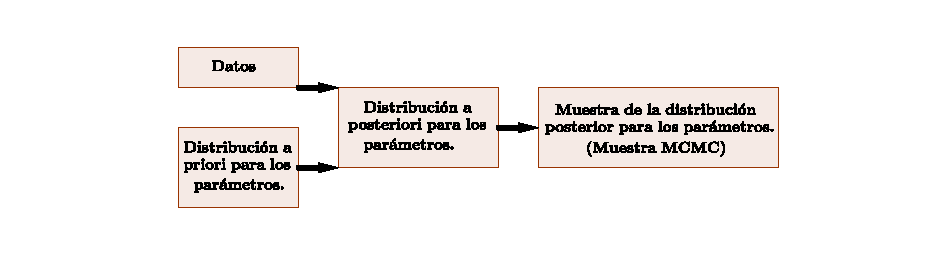
\includegraphics[scale=1.25]{esq.pdf} \\
%\end{tabular}
%\end{frame}


\begin{frame}{Construcci\'on del plan de almacenamiento}
\begin{tabular}{c}
\hspace{-5.6cm}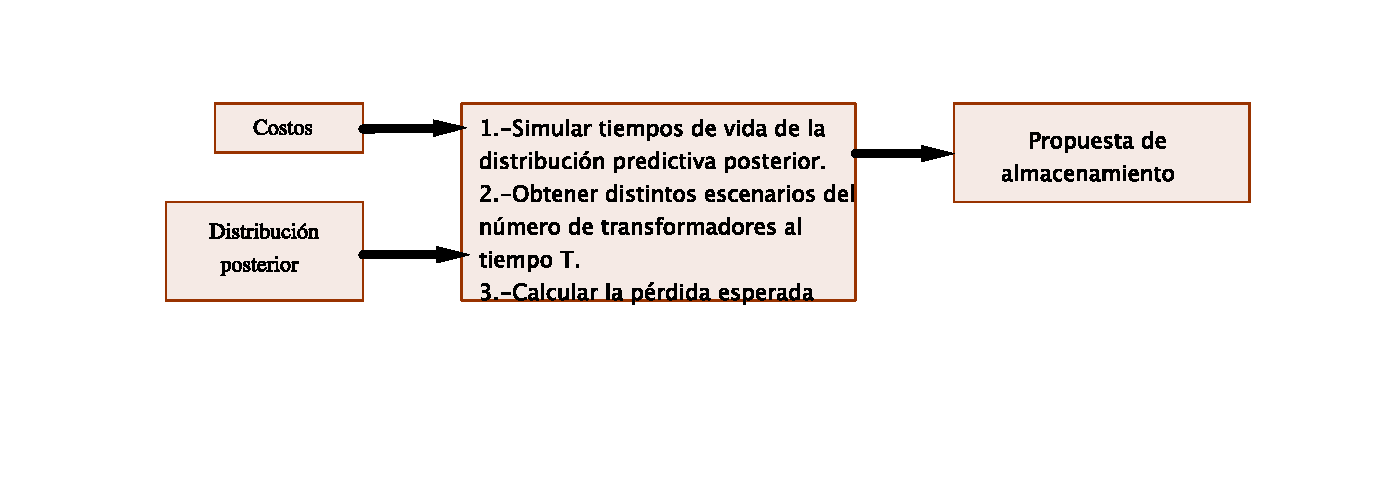
\includegraphics[scale=2]{final.pdf} \\
\end{tabular}
\end{frame}

\frame{\frametitle{Planteamiento de pol\'iticas}
\begin{itemize}
\justifying
\item [A]
La primera pol\'itica reflejar\'a el costo de quedarnos sin transformadores disponibles en el almac\'en. 
\item[B] 
La segunda pol\'itica adem\'as de considerar el costo de la pol\'itica A, adiciona el costo del lote inicial de transformadores en el almac\'en. 
\item[C] 
Esta \'ultima pol\'itica se centra en evaluar dos tipos de costos.
\begin{itemize}
\item[1.-] Costo de falta de transformadores por unidad de tiempo. Este costo tambi\'en considerado en las pol\'iticas anteriores.
\item[2.-] Costo de almacenamiento por cada unidad de tiempo.
\end{itemize}
\end{itemize}
}


\frame{\frametitle{Pol\'itica A}
\justifying
\noindent Sean $\underline{T}=\{t_1,t_2,\cdots,t_n\}$ los tiempos de falla de los transformadores y 
$\underline{\ell}=\{\ell_1=t_1+\delta, \ell_2=t_2+\delta, \cdots, \ell_n=t_n+\delta\},$ los tiempos de llegada de los transformadores pedidos. 

\noindent  Definamos  $X(t;\underline{T})$ como el  n\'umero de transformadores en el almac\'en que se usaron para cubrir los tiempos de fallas hasta el tiempo $t$ y  $Y(t;\underline{T})$ el n\'umero de transformadores que se pidieron y llegaron antes del tiempo $t$. Luego $X(0)=n_0$ y $Y(0)=0$.}

\frame{
\noindent Sea $Z(t;\underline{T})=X(t;\underline{T})+Y(t,\underline{T})$.

\noindent La siguiente funci\'on restringue solo al \'area de inter\'es 
\[
W(t;\underline{T})=\left\{
\begin{array}{cl}
\displaystyle 0 & \mbox{ si } Z(t;\underline{T})\geq 0,\\                                                               Z(t)      &     \mbox{ si } Z(t;\underline{T})< 0  \\
\end{array}
\right.
\]

\noindent Una vez establecidas las funciones anteriores la funci\'on de utilidad esta dada por 

\begin{eqnarray}\label{LL}
L(t,\underline{T},\delta, n_0)=\int_{0}^{t} W(s,\underline{T}) ds,
\end{eqnarray}
}



\frame{\frametitle{}
\justifying
\noindent La {\bf Utilidad Esperada} es
\begin{eqnarray*}
U(t,n_0,\delta)=E(L(t,\underline{T},n_0, \delta)).
\end{eqnarray*}

\noindent Por la ley de los grandes n\'umeros, la manera de estimarla es mediante la  expresi\'on:

\begin{eqnarray}\label{utqq}
\hat{U}(t,n_0,\delta)=\frac{1}{M} \sum_{s=1}^{M}\int_{0}^{t} W(y,\underline{T}_s) dy,
\end{eqnarray}
 donde $M$ es el n\'umero de $\underline{T}_s$ simulados.
}
\frame{
\justifying
\noindent Para calcular la expresi\'on (\ref{utqq}) por simulaci\'on se hace de la siguiente manera:
\begin{enumerate}
\justifying
\item Se simulan $M$ trayectorias de tiempos de vida, dicho en otras palabras $M$ vectores del tipo $\underline{T}$.
\item Para cada trayectoria se calcula la Ecuaci\'on (\ref{LL}).
\item De los $M$ valores obtenidos,  se obtiene el promedio de ellos, que ser\'a la utilidad esperada.
\end{enumerate}
}


\frame{

\noindent De acuerdo a los pasos anteriores, se realizaron 1000 simulaciones para cada pareja $$(\delta_i,n_{0_j})$$ donde $\delta_i=6, 8$ y 12 meses, $n_{0_j}=1,2,\cdots, 24$ numero de transformadores al inicio de cada periodo de observaci\'on. Luego se obtuvo el promedio de las funciones de utilidad, calculadas en cada una de las 1000 simulaciones para cada pareja.}

\frame{\frametitle{Utilidades esperadas con la pol\'itica A, usando $t=480$ y $\delta=6$}

\includegraphics[scale=0.25]{u6.pdf}

}


\frame{

\begin{table}[h!]\tiny
\centering
\caption{\bf Pol\'itica A: Valores de las utilidades esperadas con $\delta=6$.}\label{c1}
\vspace{0.3 cm}\begin{tabular}{ccccccccc}
\toprule[0.6mm]

$\bf{n_0}$&\bf{1} &                   \bf{2} &                   \bf{3} &                   \bf{ 4 }&                    \bf{ 5}&              \bf{ 6} &               \bf{ 7} & \bf{8} \\
\hline
$\mbox{\bf Promedio}$&1029.433  &697.822&  437.725&  251.263 & 131.085 &  62.514 &  27.148 &  11.136 \\	
\hline
$\bf{n_0}$&\bf{9} &                \bf{ 10}&              \bf{      11} &                   \bf{ 12} &               \bf{      13}&              \bf{14} &  \bf{ 15} & \bf{16 }   \\
\hline
$\mbox{\bf Promedio}$&	 4.003  &  1.343 &   0.446 &   0.167&    0.028 &   0.040 &   0.000&    0.000\\ 
	 \hline
	
$\bf{n_0}$&\bf{17} &     \bf{ 18}&   \bf{19}&   \bf{ 20} &           \bf{   21}&                \bf{  22}  & \bf{23} & \bf{24}  \\
\hline
$\mbox{\bf Promedio}$&  0.000 &   0.000&    0.000 &   0.000   & 0.000  &  0.000 &   0.000 & 0.000\\
\toprule[0.6mm]
\end{tabular}
\end{table}
}


\frame{\frametitle{Pol\'itica B}
\begin{description}
\justifying
\item [Costo 1:] \hfill \\El costo de no poder cobrar la electricidad durante un  periodo de tiempo donde no hab\'ia transformadores en reserva, considerado en la secci\'on anterior.
\item [Costo 2:] \hfill\\El costo de almacenamiento por unidad de tiempo.
\end{description}
\justifying
\noindent Sea $C$ el costo de no poder cobrar la electricidad en una unidad de tiempo. Luego el costo de almacenar un transformador por una unidad de tiempo, lo podemos expresar en t\'erminos de $C$ como
 $rC$. Asumiendo que el {\bf Costo 1} es mayor que el {\bf Costo 2} entonces $r \in(0,1)$.
}

\frame{

\noindent  La funci\'on de utilidad considerando el {\bf costo 1} y el costo inicial de almacenamiento durante la primera unidad de tiempo es:
\begin{eqnarray*}
L(t,\underline{T},\delta, n_0)=C\int_{0}^{t} W(s,\underline{T})  ds + rn_0C \mbox{ },
\end{eqnarray*}

\noindent Suponiendo $C=1$, es decir, una unidad de dinero. La utilidad se simplifica a: 
\begin{eqnarray}\label{LL1}
L(t,\underline{T},\delta, n_0)=\int_{0}^{t} W(s,\underline{T})  ds + rn_0,
\end{eqnarray}
La utilidad esperada puede calcularse como:
\begin{eqnarray*}
\hat{U}(t,n_0,\delta)=\frac{1}{M} \sum_{s=1}^{M}\left(\int_{0}^{t} W(y,\underline{T}_s) dy + n_0r\right)
\end{eqnarray*}

}


\frame{
\noindent Asignando valores a $r$, se puede observar la manera de comportarse de esta funci\'on de utilidad (\ref{LL1}). La manera de estimar la p\'erdida esperada es por medio de simulaciones.
}


\frame{\frametitle{Utilidades esperadas usando la pol\'itica B, con $\delta=6$ y r=0.1}

\includegraphics[scale=0.25]{utilpeso01delta6.pdf}

}

\frame{
\begin{table}[h!]\tiny
\centering
\caption{\bf Pol\'itica B: Valores de las utilidades esperadas con $\delta=6$, $r=0.1$.}\label{r11}
\begin{tabular}{ccccccccc}
\toprule[0.6mm]
$\bf{n_0}$ &\bf{1} &                   \bf{2} &                   \bf{3} &                   \bf{ 4 }&                    \bf{ 5}&              \bf{ 6} &               \bf{ 7} & \bf{8} \\
\hline
${\bf Promedio}$ &  
 1026.86 &  701.26 & 441.20 & 248.58 & 132.61  & 61.29 &  27.04&   12.30 \\
\hline
$\bf{n_0}$& \bf{9} &                \bf{ 10}&              \bf{      11} &                   \bf{ 12} &               \bf{      13}&              \bf{14} &  \bf{ 15} & \bf{16 }   \\
\hline
${\bf Promedio}$&	  5.50 &   2.71 &   1.50 &   1.39 &   1.34 &   1.43  &  1.50 &   1.60    \\
	 \hline
	
$\bf{n_0}$&\bf{17} &     \bf{ 18}&   \bf{19}&   \bf{ 20} &           \bf{   21}&                \bf{  22}  & \bf{23} & \bf{23}  \\
\hline
${\bf Promedio}$&    1.70  &1.80 &   1.90 &   2.00  &  2.10  &  2.20 &   2.30  &   2.40 \\
\toprule[0.6mm]
\end{tabular}

\end{table}

}

\frame{\frametitle{Pol\'itica C}

\noindent Esta \'ultima pol\'itica considera los dos costos empleados en la Pol\'itica B por unidad de tiempo. La funci\'on de utilidad, esta dada por la siguiente expresi\'on.
\begin{eqnarray}
L(t,\underline{T},\delta,n_0)=\int_{0}^{t} W(s,\underline{T}) ds + r \int_{0}^{t} A(s,\underline{T}) ds
\end{eqnarray}
donde:
\[
A(t,\underline{T})=\left\{
\begin{array}{cl}
\displaystyle 0 & \mbox{ si } Z(t,\underline{T})\leq 0,\\                                                               Z(t)      &     \mbox{ si } Z(t,\underline{T})>0  \\
\end{array}
\right.
\]

\noindent La funci\'on $A(t,\underline{T})$ refleja las p\'erdidas que existen por almacenar transformadores. La utilidad esperada se calcula como:
\begin{eqnarray}\label{LL3}
\hat{U}(t,n_0,\delta)&=& \frac{1}{M}\sum_{s=1}^M \left(     \int_{0}^{t} W(s,\underline{T}) ds + r \int_{0}^{t} A(s,\underline{T}) ds       \right).
\end{eqnarray}
}


\frame{\frametitle{Utilidades esperadas usando la pol\'itica C con $\delta=6$ y $r=0.01$}

\includegraphics[scale=0.25]{uA8.pdf}

}
\frame{
\begin{table}[h!]\tiny
\centering
\caption{\bf Pol\'itica C. Valores de las utilidades esperadas con $\delta=6$ y $r=0.01$.}\label{u38t}
\begin{tabular}{ccccccccc}
\toprule[0.6mm]
$\bf{n_0}$&\bf{1} &                   \bf{2} &                   \bf{3} &                   \bf{ 4 }&                    \bf{ 5}&              \bf{ 6} &               \bf{ 7} & \bf{8} \\
\hline
{\bf Promedio}& 611687.9 &413680.9 &256825.8& 150424.5&  75977.0  &37610.2 & 16419.3 &   6576.2  \\
\hline
$\bf{n_0}$&\bf{9} &                \bf{ 10}&              \bf{      11} &                   \bf{ 12} &               \bf{      13}&              \bf{14} &  \bf{ 15} & \bf{16 }   \\
\hline
{\bf Promedio}&	    2408.7  & 1021.0 &   190.9 &   140.7 & 138.1  &  117.3  &  114.6 &   124.0  \\
	 \hline
	
$\bf{n_0}$&\bf{17} &     \bf{ 18}&   \bf{19}&   \bf{ 20} &           \bf{   21}&                \bf{  22}  & \bf{23} &  \bf{24}\\
\hline
{\bf Promedio}&  133.4 &   144.0 &152.2    &163.5 &   172.2  &  180.6 &   190.4 &199.2\\
\toprule[0.6mm]
\end{tabular}
\end{table}
}
%\section{Conclusiones}
\frame{\frametitle{Conclusiones}

Se han descrito 3 pol\'iticas de almacenamiento, que pretender crear entornos realistas, para determinar los valores \'optimos que conduzcan a la minimizaci\'on de costos. A continuaci\'on se muestran los resultados resumidos obtenidos.

}

\frame{\frametitle{Conclusiones}
\begin{table}[h!]\small
\begin{center}
\caption{\bf Resultados de la pol\'itica A.}\label{taba1}
\vspace{0.3cm}
\begin{tabular}{ccc}
\toprule[0.6mm]
  $\delta$ & $n_0$ & costo\\
\toprule[0.6mm]
  6 & 15 &0.00\\
  8&19& 0.00\\
  12&24 & 0.00\\
\toprule[0.6mm]
\end{tabular}
\end{center}
\end{table}
}


\frame{
\begin{table}[ht]\tiny
\begin{center}
\caption{\bf Resultados de la pol\'itica B.}
\vspace{0.3cm}
\begin{tabular}{cccc}
\toprule[0.6mm]
 $\delta$ & $n_0$  & costo& $r$\\
\toprule[0.6mm]
  6   & 14 & 0.14& 0.01\\
  8   & 17 & 0.16& 0.01\\
  12 & 22  & 0.20 & 0.01\\
  \hline
  6   & 13 & 1.34& 0.1\\
  8   & 14 & 1.49& 0.1\\
  12 & 20 & 2.00& 0.1\\
  \hline
  6   & 11& 5.65 &0.5 \\
  8   & 14 &7.11 & 0.5 \\
  12 & 18 &9.16 &0.5\\
\toprule[0.6mm]
\end{tabular}
\end{center}
\end{table}
}

\frame{
\begin{table}[h!]\tiny
\begin{center}
\caption{\bf Resultados de la pol\'itica C.}\label{resuFF}
\vspace{0.3cm}\begin{tabular}{cccc}
\toprule[0.6mm]
 $\delta$ & $n_0$  & costo& $r$\\
\toprule[0.6mm]
  6   & 15 & 114& 0.01\\
  8   & 16 & 119& 0.01\\
  12 & 20  & 145 & 0.01\\
  \hline
  6   & 12 & 526& 0.1\\
  8   & 15 & 606& 0.1\\
  12 & 20 & 779& 0.1\\
  \hline
  6   & 11& 2209&0.5 \\
  8   & 14&2524 & 0.5 \\
  12 & 15 &8836 &0.5\\
\toprule[0.6mm]
\end{tabular}
\end{center}
\end{table}}



\frame{
\begin{itemize}
\item Una vez presentadas las funciones de utilidad planteadas y los resultados obtenidos. La pregunta de inter\'es es ?`C\'ual es la m\'as adecuada?, la aplicaci\'on de cualquiera de ellas depender\'a de las condiciones reales de problema.
\end{itemize}}

\frame{
El objetivo principal de este trabajo, fue proponer una pol\'itica de inventario de transformadores de instrumento, empleando herramientas de estad\'istica Bayesiana. El esquema muestra el panorama general utilizado.

\begin{tabular}{c}
\hspace{-2cm}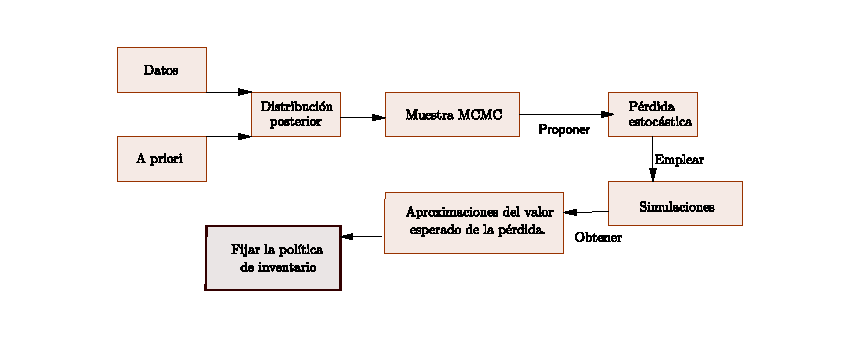
\includegraphics[scale=1]{resumen.pdf} \\
\end{tabular}
}


\frame{\frametitle{Bibliograf\'ia}
\begin{thebibliography}{99}
%\beamertemplatebookbibitems para que se ponga el librito indicando que es un libro a loq ue se hace referencia.
\beamertemplatearticlebibitems % para que se ponga el cuadernillo de articulo
\bibitem{riesgo} Peter M. Lee. \textbf{``Bayesian Statistics an introduction''}. Wiley series in Probability and Mathematical Statistic ,3 edici\'on (2004). \label{PL}

\bibitem{riesgo} William Q. Meeker and Luis A. Escobar. \textbf{``Statistical Metohds for Reliability Data''}. Wiley series in Probability and Mathematical Statistic (1998). \label{me}

\bibitem{Grandell} Michael S. Hamada Alyson G. Wilson, C. Shane Reese Harry F. Martz \textbf{``Bayesian Reliability''}. Springer-Science+Bisiness (2008).\label{BR}
\end{thebibliography}}

\frame{
\begin{center}
GRACIAS
\end{center}
}
\end{document}







